\newcommand{\titulus}{\nomenFesti{Dominica XXVII per Annum.}}
\newcommand{\tedeummonasticum}{Monasticum}
\newcommand{\oratio}{\pars{Oratio.}

\noindent Omnípotens sempitérne Deus, qui abundántia pietátis tuæ et mérita súpplicum excédis et vota, effúnde super nos misericórdiam tuam, ut dimíttas quæ consciéntia métuit et adícias quod orátio non præsúmit.

\pars{Pro pace in Ucraina.} \scriptura{Sir. 50, 25; 2 Esdr. 4, 20; \textbf{H416}}

\vspace{-4mm}

\antiphona{II D}{temporalia/ant-dapacemdomine.gtex}

\vfill

\noindent Deus, a quo sancta desidéria, recta consília et iusta sunt ópera: da servis tuis illam, quam mundus dare non potest, pacem; ut et corda nostra mandátis tuis dédita, et hóstium subláta formídine, témpora sint tua protectióne tranquílla.

\noindent Per Dóminum nostrum Iesum Christum, Fílium tuum, qui tecum vivit et regnat in unitáte Spíritus Sancti, Deus, per ómnia sǽcula sæculórum.

\noindent \Rbardot{} Amen.}
\newcommand{\nocturnoi}{\pars{Psalmus 1.} \scriptura{Ps. 1, 2; \textbf{H372}}

\vspace{-4mm}

\antiphona{I d}{temporalia/ant-inlegedominifuit.gtex}

%\vspace{-2mm}

\scriptura{Ps. 1}

%\vspace{-2mm}

\initiumpsalmi{temporalia/ps1-initium-i-d-auto.gtex}

\input{temporalia/ps1-i-d.tex} \Abardot{}

\vfill
\pagebreak

\pars{Psalmus 2.} \scriptura{Ps. 2, 6; \textbf{H372}}

\vspace{-4mm}

\antiphona{III a}{temporalia/ant-praedicanspraeceptumdomini.gtex}

\vspace{-1mm}

\scriptura{Ps. 2}

\vspace{-2mm}

\initiumpsalmi{temporalia/ps2-initium-iii-a-auto.gtex}

\input{temporalia/ps2-iii-a.tex} \Abardot{}

\vfill
\pagebreak

\pars{Psalmus 3.} \scriptura{Ps. 3, 5; \textbf{H372}}

\vspace{-4mm}

\antiphona{VII c trans.}{temporalia/ant-vocemeaaddominum.gtex}

%\vspace{-2mm}

\scriptura{Ps. 3}

\initiumpsalmi{temporalia/ps3-initium-vii-c-trans.gtex}

\input{temporalia/ps3-vii-c.tex} \Abardot{}

\vfill
\pagebreak
}
\newcommand{\nocturnoii}{\vspace{-4mm}

\pars{Psalmus 4.} \scriptura{Ex. 15, 2; \textbf{H39}}

\vspace{-4mm}

\antiphona{VIII G}{temporalia/ant-eccedeusmeus.gtex}

%\vspace{-2mm}

\scriptura{Ps. 144, 1-9}

%\vspace{-2mm}

\initiumpsalmi{temporalia/ps144i-initium-viii-G-auto.gtex}

\input{temporalia/ps144i-viii-G.tex} \Abardot{}

\vfill
\pagebreak

\pars{Psalmus 5.} \scriptura{Ps. 144, 13; \textbf{H100}}

\vspace{-4mm}

\antiphona{VII c}{temporalia/ant-regnumtuumdomine.gtex}

%\vspace{-2mm}

\scriptura{Ps. 144, 10-13}

\initiumpsalmi{temporalia/ps144x_xiii-initium-vii-c-auto.gtex}

\input{temporalia/ps144x_xiii-vii-c.tex} \Abardot{}

\vfill
\pagebreak

\pars{Psalmus 6.} \scriptura{\textbf{H99}}

\vspace{-4mm}

\antiphona{VIII a}{temporalia/ant-inaeternumet.gtex}

%\vspace{-4mm}

\scriptura{Ps. 144, 14-21}

%\vspace{-2mm}

\initiumpsalmi{temporalia/ps144xiv_xxi-initium-viii-a-auto.gtex}

%\vspace{-1.5mm}

\input{temporalia/ps144xiv_xxi-viii-a.tex} \Abardot{}

\vfill
\pagebreak}
\newcommand{\nocturnoiii}{\pars{Cantica.}

\vspace{-4mm}

\antiphona{D}{temporalia/ant-eccedeusnoster.gtex}

%\vspace{-2mm}

\scriptura{Canticum Isaiæ, Is. 33, 2-10}

%\vspace{-2mm}

\initiumpsalmi{temporalia/isaiae7-initium-d-g-auto.gtex}

\input{temporalia/isaiae7-d-g.tex} \hfill \rubrica{Hic non dicitur antiphona.}

\vfill
\pagebreak

\scriptura{Canticum Isaiæ, Is. 33, 13-17}

%\vspace{-2mm}

\initiumpsalmi{temporalia/isaiae8-initium-d-g-auto.gtex}

\input{temporalia/isaiae8-d-g.tex}

\vfill
\pagebreak

\scriptura{Canticum Ecclesiastici, Sir. 36, 14-19}

%\vspace{-2mm}

\initiumpsalmi{temporalia/ecclesiasticus36-initium-d-g-auto.gtex}

\input{temporalia/ecclesiasticus36-d-g.tex}

\vfill

\antiphona{}{temporalia/ant-eccedeusnoster.gtex}

\vfill
\pagebreak}
\newcommand{\lectioi}{\pars{Lectio I.} \scriptura{1 Tim. 1, 1-7}

\noindent Incipit Epístola prima beáti Pauli apóstoli ad Timótheum.

\noindent Paulus apóstolus Christi Iesu secúndum præcéptum Dei salvatóris nostri et Christi Iesu spei nostræ, Timótheo, germáno fílio in fide: grátia, misericórdia, pax a Deo Patre et Christo Iesu Dómino nostro.

\noindent Sicut rogávi te, ut remanéres Ephesi, cum irem in Macedóniam, ut præcíperes quibúsdam, ne áliter docérent, neque inténderent fábulis et genealogíis interminátis, quæ quæstiónes præstant magis quam dispensatiónem Dei, quæ est in fide; finis autem præcépti est cáritas de corde puro et consciéntia bona et fide non ficta, a quibus quidam aberrántes convérsi sunt in vanilóquium, voléntes esse legis doctóres, non intellegéntes neque quæ loquúntur neque de quibus affírmant.}
\newcommand{\responsoriumi}{\pars{Responsorium 1.} \scriptura{\Rbardot{} Ps. 15, 10 \Vbardot{} ibid., 1; \textbf{H83}}

\vspace{-5mm}

\responsorium{VIII}{temporalia/resp-notasmihifecisti-CROCHU.gtex}{}}
\newcommand{\lectioii}{\pars{Lectio II.} \scriptura{1 Tim. 1, 8-14}

\noindent Scimus autem quia bona est lex, si quis ea legítime utátur, sciens hoc quia iusto lex non est pósita, sed iniústis et non subiéctis, ímpiis et peccatóribus, scelerátis et contaminátis, patricídis et matricídis, homicídis, fornicáriis, masculórum concubitóribus, plagiáriis, mendácibus, periúris, et si quid áliud sanæ doctrínæ adversátur, secúndum evangélium glóriæ beáti Dei, quod créditum est mihi.

\noindent Grátiam hábeo ei, qui me confortávit, Christo Iesu Dómino nostro, quia fidélem me existimávit ponens in ministério, qui prius fui blasphémus et persecútor et contumeliósus; sed misericórdiam consecútus sum, quia ignórans feci in incredulitáte, superabundávit autem grátia Dómini nostri cum fide et dilectióne, quæ sunt in Christo Iesu.}
\newcommand{\responsoriumii}{\pars{Responsorium 2.} \scriptura{\textbf{H84}}

\vspace{-5mm}

\responsorium{VIII}{temporalia/resp-afflictipropeccatisnostris-CROCHU.gtex}{}}
\newcommand{\lectioiii}{\pars{Lectio III.} \scriptura{1 Tim. 1, 15-20}

\noindent Fidélis sermo et omni acceptióne dignus: Christus Iesus venit in mundum peccatóres salvos fácere; quorum primus ego sum, sed ídeo misericórdiam consecútus sum, ut in me primo osténderet Christus Iesus omnem longanimitátem, ad informatiónem eórum, qui creditúri sunt illi in vitam ætérnam.

\noindent Regi autem sæculórum, incorruptíbili, invisíbili, soli Deo honor et glória in sǽcula sæculórum. Amen.

\noindent Hoc præcéptum comméndo tibi, fili Timóthee, secúndum præcedéntes super te prophetías, ut mílites in illis bonam milítiam habens fidem et bonam consciéntiam, quam quidam repelléntes circa fidem naufragavérunt; ex quibus est Hymenǽus et Alexánder, quos trádidi Sátanæ, ut discant non blasphemáre.}
\newcommand{\responsoriumiii}{\pars{Responsorium 3.} \scriptura{\Rbardot{} Ps. 15, 8-9 \Vbardot{} ibid., 1-2; \textbf{H83}}

\vspace{-5mm}

\responsorium{VIII}{temporalia/resp-adextrisestmihi-CROCHU-cumdox.gtex}{}}
\newcommand{\lectioiv}{\pars{Lectio IV.} \scriptura{Lib. 2, 4: PL 77, 30-31}

\noindent E Régula pastoráli sancti Gregórii Magni papæ.

\noindent Sit rector discrétus in siléntio, útilis in verbo, ne aut tacénda próferat aut proferénda reticéscat. Nam sicut incáuta locútio in errórem pértrahit, ita indiscrétum siléntium hos qui erudíri póterant, in erróre derelínquit. Sæpe namque rectóres impróvidi humánam amíttere grátiam formidántes, loqui líbere recta pertiméscunt; et iuxta Veritátis vocem, nequáquam iam gregis custódiæ pastórum stúdio, sed mercenariórum vice desérviunt, quia veniénte lupo fúgiunt, dum se sub siléntio abscóndunt.

\noindent Hinc namque eos per Prophétam Dóminus íncrepat, dicens: \textit{Canes muti non valéntes latráre.} Hinc rursum quéritur dicens: \textit{Non ascendístis ex advérso, nec opposuístis murum pro domo Israel, ut starétis in prœ́lio in die Dómini.} Ex advérso quippe ascéndere, est pro defensióne gregis voce líbera huius mundi potestátibus contraíre. Et in die Dómini in pr\'{œ}lio stare, est pravis decertántibus ex iustítiæ amóre resístere.}
\newcommand{\responsoriumiv}{\pars{Responsorium 4.} \scriptura{\Rbardot{} Ps. 6, 1-2 \Vbardot{} Ps. 54, 6-7; \textbf{H83}}

\vspace{-5mm}

\responsorium{I}{temporalia/resp-domineneiniratua-CROCHU.gtex}{}}
\newcommand{\lectiov}{\pars{Lectio V.}

\noindent Pastóri enim recta timuísse dícere, quid est áliud quam tacéndo terga præbuísse? qui nimírum si pro grege se óbicit, murum pro domo Israel hóstibus oppónit. Hinc rursum delinquénti pópulo dícitur: \textit{Prophétæ tui vidérunt tibi falsa et stulta, nec aperiébant iniquitátem tuam, ut te ad pæniténtiam provocárent.} Prophétæ quippe in sacro elóquio nonnúmquam doctóres vocántur, qui dum fugitíva esse præséntia índicant, quæ sunt ventúra maniféstant. Quos divínus sermo falsa vidére redárguit, quia dum corrípere culpas métuunt, incássum delinquéntibus promíssa securitáte blandiúntur; qui iniquitátem peccántium nequáquam apériunt quia ab increpatiónis voce conticéscunt.}
\newcommand{\responsoriumv}{\pars{Responsorium 5.} \scriptura{\Rbardot{} Ps. 25, 7 \Vbardot{} ibid., 8; \textbf{H84}}

\vspace{-5mm}

\responsorium{VII}{temporalia/resp-audiamdomine-CROCHU.gtex}{}}
\newcommand{\lectiovi}{\pars{Lectio VI.}

\noindent Clavis quippe apertiónis est sermo correptiónis, quia increpándo culpam détegit, quam sæpe nescit ipse étiam qui perpetrávit. Hinc Paulus ait: \textit{Ut potens sit exhortári in doctrína sana, et eos qui contradícunt argúere.} Hinc per Malachíam dícitur: \textit{Lábia sacerdótis custódient sciéntiam et legem requírent ex ore eius, quia ángelus Dómini exercítuum est.} Hinc per Isaíam Dóminus ádmonet, dicens: \textit{Clama, ne cesses, quasi tuba exálta vocem tuam.}

\noindent Præcónis quippe offícium súscipit quisquis ad sacerdótium accédit, ut ante advéntum iúdicis qui terribíliter séquitur, ipse scílicet clamándo gradiátur. Sacérdos ergo si prædicatiónis est néscius, quam clamóris vocem datúrus est præco mutus? Hinc est enim quod super pastóres primos in linguárum spécie Spíritus Sanctus insédit: quia nimírum quos repléverit, de se prótinus loquéntes facit.}
\newcommand{\responsoriumvi}{\pars{Responsorium 6.} \scriptura{\Rbardot{} Ps. 118, 173 \Vbardot{} ibid., 176; \textbf{H85}}

\vspace{-5mm}

\responsorium{IV}{temporalia/resp-fiatmanustua-CROCHU-cumdox.gtex}{}}
\newcommand{\evangelium}{
\pars{Versus.} \scriptura{Ps. 118, 148}

% Versus. %%%
\sineinitiali{temporalia/versus-praevenerunt.gtex}

\vspace{5mm}

\sineinitiali{temporalia/oratiodominica-mat.gtex}

\vspace{5mm}

\pars{Absolutio.}

\cuminitiali{}{temporalia/absolutio-avinculis.gtex}

\vfill
\pagebreak

\cuminitiali{}{temporalia/benedictio-solemn-evangelica.gtex}

\vspace{7mm}

\pars{Evangelium} \scriptura{Mt. 21, 33-43}

\noindent Léctio sancti Evangélii secúndum Matthǽum.

\noindent In illo témpore: Dixit Iesus princípibus sacerdótum et senióribus pópuli:

\noindent «Aliam parábolam audíte. Homo erat pater famílias, qui plantávit víneam et sæpem circúmdedit ei et fodit in ea tórcular et ædificávit turrim et locávit eam agrícolis et péregre proféctus est.

\noindent Cum autem tempus frúctuum appropinquásset, misit servos suos ad agrícolas, ut accíperent fructus eius. Et agrícolæ, apprehénsis servis eius, álium cecidérunt, álium occidérunt, álium vero lapidavérunt. Iterum misit álios servos plures prióribus, et fecérunt illis simíliter.

\noindent Novíssime autem misit ad eos fílium suum dicens: “Verebúntur fílium meum”. Agrícolæ autem vidéntes fílium dixérunt intra se: “Hic est heres. Veníte, occidámus eum et habébimus hereditátem eius”. Et apprehénsum eum eiecérunt extra víneam et occidérunt.

\noindent Cum ergo vénerit dóminus víneæ, quid fáciet agrícolis illis?».

\noindent Aiunt illi: «Malos male perdet et víneam locábit áliis agrícolis, qui reddant ei fructum tempóribus suis».

\noindent Dicit illis Iesus: «Numquam legístis in Scriptúris: “Lápidem quem reprobavérunt ædificántes, hic factus est in caput ánguli; a Dómino factum est istud et est mirábile in óculis nostris”? Ideo dico vobis quia auferétur a vobis regnum Dei et dábitur genti faciénti fructus eius. Et, qui cecíderit super lápidem istum confringétur; super quem vero cecíderit, cónteret eum».

\scriptura{Cap. 21, lect. 2 : ed. Marietti, 267. 268, vel ed. Parmæ, t. X, 196.197}

\noindent Ex Commentário sancti Thomæ de Aquíno presbýteri super Evangélium Matthǽi.

\noindent \emph{Homo erat paterfamílias, qui plantávit víneam.} Símile pónitur, ubi dícitur: \emph{Vínea facta est dilécto meo in cornu fílio ólei.} Dicunt áliqui quod ibi invéhitur contra víneam, unde dicit: \emph{Quid ultra débui fácere víneæ meæ?} Hic autem contra agrícolas.

\noindent Vínea dícitur pópulus iudáicus: \emph{Vínea Dómini domus Israel est.} Quod contra agrícolas: quia quantum ad præsens huius malítia non procéssit ex pópulo, sed ex princípibus: \emph{Numquid áliqui ex princípibus credidérunt in eum?} Ideo non contra víneam. Hæc vínea non est domus Israel [tantum], sed [étiam] iustítia Dei, quæ occúlte trádita est in sacra Scriptúra; unde dicit: \emph{paterfamílias plantávit víneam,} id est pópulum iudáicum, secúndum hoc psalmum: \emph{Víneam de Ægýpto transtulísti.} Vel iustítiam pósuit in doctrína legis.

\noindent \emph{Et sæpem circúmdedit ei,} ad protectiónem víneæ; unde quæ ponúntur ad custódiam, sive sint oratiónes sanctórum, vel custódia angelórum, dicúntur sæpes.

\noindent Si autem vínea dicátur iustítia, sæpe dicit occúlta verba Scriptúræ. \emph{Et fodit in ea tórcular.} Tórcular pónitur ut exprimátur vinum caritátis.

\noindent Si intellegátur per víneam iudáicus pópulus, intellégitur per tórcular altáre holocaustórum. Item intellegúntur mártyres, qui pro fide sánguinem fudérunt. Vel potest étiam intellégi ordo prophetárum, in quibus vinum sapiéntiæ est expréssum. Vel potest dici profúnditas sacræ Scriptúræ. Item totus fructus víneæ congregátur in torculári; sic quidquid potest ánimus, totum debet congregáre ad laudem Dei.

\noindent {\color{gray} \emph{Et ædificávit turrim.} Per turrim templum intellégitur. Vel cognítio Dei: \emph{Turris fortíssima nomen Dómini.} — Et \emph{locávit eam agrícolis.} Agrícolæ sunt, qui præponúntur pópulo.

\noindent \emph{Proféctus est péregre} Dóminus, non mutándo locum, sed hóminem in suo arbítrio reliquéndo. \emph{Cum autem tempus frúctuum appropinquásset:} quicúmque facit áliquem fructum, exspéctat benefícium; et sic Dóminus exspéctat ut reddátur ei benefícium ad suam glóriam.

\noindent \emph{Misit servos suos,} id est prophétas \emph{ad agrícolas,} ut indúcerent hómines ad bene agéndum. Sed \emph{occidérunt} eos.

\noindent \emph{Iterum misit álios.} Item singuláriter misit prophétas ut Móysen, et Aaron, et álios. Vult enim Dóminus pugnáre misericórdiam suam contra malítiam eórum.

\noindent \emph{Misit ad eos fílium suum dicens: «Forte verebúntur fílium meum.»}

\noindent Ipse enim Fílius vere heres est Patris, quia quod petit óbtinet: \emph{Póstula a me, et dabo tibi gentes hereditátem tuam.}Item est heres quia quæcúmque habet Pater, habet et ipse. Sed contra: \emph{Si cognovíssent, numquam Dóminum glóriæ crucifixíssent.} Verum est, si cognovíssent vere; sed cognovérunt per coniectúram.

\noindent Séquitur propósitum: \emph{Veníte, occidámus eum. — Dóminus víneæ, quid fáciet agrícolis illis?} Ita subtíliter petit Dóminus ut iúdicent contra se, sicut Nathan fecit David; \emph{aiunt illi: «Malos male perdet.»} Item verum est quod príncipes dixérunt. Et quamvis percíperent quod contra eos esset, non contradicébant.

\noindent \emph{Dicit illis Iesus: «Lápidem quem reprobavérunt ædificántes, hic factus est in caput ánguli.»} Lapis Christus est; et constitútus est in caput ánguli, id est in caput Iudæórum et gentílium. Unde ipse factus est caput Ecclésiæ. \emph{Et est mirábile in óculis nostris.}}

\vfill
\pagebreak

\pars{Responsorium 7.} \scriptura{\Rbardot{} Ps. 54, 10 \Vbardot{} Ier. 14, 19; \textbf{H419}}

\vspace{-5mm}

\responsorium{III}{temporalia/resp-praecipitadomine-CROCHU-cumdox.gtex}{}

\rubrica{vel ad libitum:}

\vspace{3mm}

\pars{Responsorium 7.} \scriptura{\Rbardot{} Cantor \Vbardot{} Dan. 19, 16; \textbf{H419}}

\vspace{-5mm}

\responsorium{II}{temporalia/resp-civitatemistamtucircumda-CROCHU-cumdox.gtex}{}

\vfill
\pagebreak
}
\newcommand{\responsoriumbreve}{\pars{Responsorium breve.}

\cuminitiali{VI}{temporalia/resp-christefilidei.gtex}}
\newcommand{\benedictus}{\pars{Canticum Zachariæ.} \scriptura{Mt. 21, 41; \textbf{H153}}

\vspace{-4mm}

{
\grechangedim{interwordspacetext}{0.18 cm plus 0.15 cm minus 0.05 cm}{scalable}%
\antiphona{III a\textsuperscript{2}}{temporalia/ant-malosmaleperdet.gtex}
\grechangedim{interwordspacetext}{0.22 cm plus 0.15 cm minus 0.05 cm}{scalable}%
}

%\vspace{-3mm}

\scriptura{Lc. 1, 68-79}

%\vspace{-2mm}

\initiumpsalmi{temporalia/benedictus-initium-iiisoll-a4-auto.gtex}

%\vspace{-1.5mm}

\input{temporalia/benedictus-iiisoll-a4.tex}

\vfill

{
\grechangedim{interwordspacetext}{0.18 cm plus 0.15 cm minus 0.05 cm}{scalable}%
\antiphona{}{temporalia/ant-malosmaleperdet.gtex}
\grechangedim{interwordspacetext}{0.22 cm plus 0.15 cm minus 0.05 cm}{scalable}%
}
}
\newcommand{\hebdomada}{infra Hebdom. XXIII per Annum.}
\newcommand{\hiemalis}{Hiemalis}
\newcommand{\matuc}{Matutinum Hebdomadae C}
\newcommand{\matuac}{Matutinum Hebdomadae A vel C}
\newcommand{\laudc}{Laudes Hebdomadae C}
\newcommand{\laudac}{Laudes Hebdomadae A vel C}

% LuaLaTeX

\documentclass[a4paper, twoside, 12pt]{article}
\usepackage[latin]{babel}
%\usepackage[landscape, left=3cm, right=1.5cm, top=2cm, bottom=1cm]{geometry} % okraje stranky
%\usepackage[landscape, a4paper, mag=1166, truedimen, left=2cm, right=1.5cm, top=1.6cm, bottom=0.95cm]{geometry} % okraje stranky
\usepackage[landscape, a4paper, mag=1400, truedimen, left=0.5cm, right=0.5cm, top=0.5cm, bottom=0.5cm]{geometry} % okraje stranky

\usepackage{fontspec}
\setmainfont[FeatureFile={junicode.fea}, Ligatures={Common, TeX}, RawFeature=+fixi]{Junicode}
%\setmainfont{Junicode}

% shortcut for Junicode without ligatures (for the Czech texts)
\newfontfamily\nlfont[FeatureFile={junicode.fea}, Ligatures={Common, TeX}, RawFeature=+fixi]{Junicode}

\usepackage{multicol}
\usepackage{color}
\usepackage{lettrine}
\usepackage{fancyhdr}

% usual packages loading:
\usepackage{luatextra}
\usepackage{graphicx} % support the \includegraphics command and options
\usepackage{gregoriotex} % for gregorio score inclusion
\usepackage{gregoriosyms}
\usepackage{wrapfig} % figures wrapped by the text
\usepackage{parcolumns}
\usepackage[contents={},opacity=1,scale=1,color=black]{background}
\usepackage{tikzpagenodes}
\usepackage{calc}
\usepackage{longtable}
\usetikzlibrary{calc}

\setlength{\headheight}{14.5pt}

% Commands used to produce a typical "Conventus" booklet

\newenvironment{titulusOfficii}{\begin{center}}{\end{center}}
\newcommand{\dies}[1]{#1

}
\newcommand{\nomenFesti}[1]{\textbf{\Large #1}

}
\newcommand{\celebratio}[1]{#1

}

\newcommand{\hora}[1]{%
\vspace{0.5cm}{\large \textbf{#1}}

\fancyhead[LE]{\thepage\ / #1}
\fancyhead[RO]{#1 / \thepage}
\addcontentsline{toc}{subsection}{#1}
}

% larger unit than a hora
\newcommand{\divisio}[1]{%
\begin{center}
{\Large \textsc{#1}}
\end{center}
\fancyhead[CO,CE]{#1}
\addcontentsline{toc}{section}{#1}
}

% a part of a hora, larger than pars
\newcommand{\subhora}[1]{
\begin{center}
{\large \textit{#1}}
\end{center}
%\fancyhead[CO,CE]{#1}
\addcontentsline{toc}{subsubsection}{#1}
}

% rubricated inline text
\newcommand{\rubricatum}[1]{\textit{#1}}

% standalone rubric
\newcommand{\rubrica}[1]{\vspace{3mm}\rubricatum{#1}}

\newcommand{\notitia}[1]{\textcolor{red}{#1}}

\newcommand{\scriptura}[1]{\hfill \small\textit{#1}}

\newcommand{\translatioCantus}[1]{\vspace{1mm}%
{\noindent\footnotesize \nlfont{#1}}}

% pruznejsi varianta nasledujiciho - umoznuje nastavit sirku sloupce
% s prekladem
\newcommand{\psalmusEtTranslatioB}[3]{
  \vspace{0.5cm}
  \begin{parcolumns}[colwidths={2=#3}, nofirstindent=true]{2}
    \colchunk{
      \input{#1}
    }

    \colchunk{
      \vspace{-0.5cm}
      {\footnotesize \nlfont
        \input{#2}
      }
    }
  \end{parcolumns}
}

\newcommand{\psalmusEtTranslatio}[2]{
  \psalmusEtTranslatioB{#1}{#2}{8.5cm}
}


\newcommand{\canticumMagnificatEtTranslatio}[1]{
  \psalmusEtTranslatioB{#1}{temporalia/extra-adventum-vespers/magnificat-boh.tex}{12cm}
}
\newcommand{\canticumBenedictusEtTranslatio}[1]{
  \psalmusEtTranslatioB{#1}{temporalia/extra-adventum-laudes/benedictus-boh.tex}{10.5cm}
}

% volne misto nad antifonami, kam si zpevaci dokresli neumy
\newcommand{\hicSuntNeumae}{\vspace{0.5cm}}

% prepinani mista mezi notovymi osnovami: pro neumovane a neneumovane zpevy
\newcommand{\cantusCumNeumis}{
  \setgrefactor{17}
  \global\advance\grespaceabovelines by 5mm%
}
\newcommand{\cantusSineNeumas}{
  \setgrefactor{17}
  \global\advance\grespaceabovelines by -5mm%
}

% znaky k umisteni nad inicialu zpevu
\newcommand{\superInitialam}[1]{\gresetfirstlineaboveinitial{\small {\textbf{#1}}}{\small {\textbf{#1}}}}

% pars officii, i.e. "oratio", ...
\newcommand{\pars}[1]{\textbf{#1}}

\newenvironment{psalmus}{
  \setlength{\parindent}{0pt}
  \setlength{\parskip}{5pt}
}{
  \setlength{\parindent}{10pt}
  \setlength{\parskip}{10pt}
}

%%%% Prejmenovat na latinske:
\newcommand{\nadpisZalmu}[1]{
  \hspace{2cm}\textbf{#1}\vspace{2mm}%
  \nopagebreak%

}

% mode, score, translation
\newcommand{\antiphona}[3]{%
\hicSuntNeumae
\superInitialam{#1}
\includescore{#2}

#3
}
 % Often used macros
%%%% Preklady jednotlivych zpevu (nektere se opakuji, a je dobre mit je
% vsechny na jedne hromade)

\newcommand{\trOratioAnteOfficium}{\translatioCantus{Otevři, Pane, má ústa, abych chválil tvé svaté jméno.
Očisti mé srdce od všech marnivých, zvrácených a~jiných myšlenek, osvěť rozum, rozněť cit,
abych mohl důstojně, soustředěně a~zbožně recitovat a~vysloužil si být
vyslyšen před tváří tvé velebnosti. Skrze Krista…}}

\newcommand{\trOratioPostOfficium}{\translatioCantus{\textit{Následující modlitbu
opatřil pro ty, kdo ji zbožně vyřknou po hodinkách, zesnulý papež Lev X.
odpustky za hříchy vzniklé při konání hodinek z~lidské křehkosti. Říká se
vkleče.}
Svatosvaté a~nerozdílné Trojici, ukřižovanému lidství našeho Pána Ježíše
Krista, přeblažené a~přeslavné plodné neporušenosti vždy Panny Marie
i~souhrnu všech svatých buď ode všeho stvoření věčná chvála, čest a~sláva, nám
pak buď dáno odpuštění všech hříchů, po nekonečné věky věků. Amen.}}

% HOURS ---

\newcommand{\trAntI}{\translatioCantus{Jasné narození slavné Panny Marie,
z pokolení (dosl. ze semene) Abrahámova, vzešlé z kmene Judova, z rodu Davidova.}}
\newcommand{\trAntII}{\translatioCantus{Dnes je Narození svaté Panny 
Marie, jejíž předrahý život osvěcuje všechny církve.}}

\newcommand{\trAntIII}{\translatioCantus{Maria, jež vzešla 
z královského rodu, září; myslí i duchem ji zbožně prosíme, aby 
nám pomáhala svými přímluvami.}}

\newcommand{\trAntIV}{\translatioCantus{Srdcem i duchem pějme Kristu 
k slávě o této svaté slavnosti vznešené Rodičky Boží Marie.}}

\newcommand{\trAntV}{\translatioCantus{Příjemně \notitia{?} 
oslavujme Narození blahoslavené Marie,
aby se ona za nás přimlouvala u Pána Ježíše Krista.}}

\newcommand{\trCapituli}{\translatioCantus{Před věky, na počátku mě stvořil, potrvám věčně. Ve svatém Stanu jsem před ním konala službu.}}

\newcommand{\trRespVesp}{\translatioCantus{Buď zdráva, Maria,
plná milosti: \grestar{} Pán s tebou. \Vbardot{} Požehnaná jsi mezi ženami,
a požehnaný plod života (ve smyslu lůna, břicha) tvého.}}

\newcommand{\trVersus}{\translatioCantus{\Vbardot{} Dnes je Narození svaté Panny Marie. \Rbardot{} Jejíž předrahý život osvěcuje všechny církve.}}

\newcommand{\trAntMagnificatI}{\translatioCantus{Konejme památku
veledůstojného narození slavné Panny Marie,
jíž se dostalo mateřské důstojnosti bez ztráty panenské cudnosti.}}

% Tento preklad je vice nez nejisty a ani alternativy, ktere jsem
% videl, me nepresvedcily...
\newcommand{\trAntBenedictus}{\translatioCantus{Slavnostně slavme 
dnešní narození Marie, vždy Panny a Rodičky Boží: v něm se objevuje
vysokost trůnu (totiž Marie, trůnu Božího Syna), aleluja.}}

\newcommand{\trAntMagnificatII}{\translatioCantus{Tvé narození,
Bohorodičko Panno, vyhlásilo radost celému světu:
z tebe totiž vzešlo Slunce spravedlnosti, Kristus, náš Bůh:
jenž zrušil kletbu a dal nám požehnání: přemohl smrt a dal nám život věčný.}}

\newcommand{\trOrationis}{\translatioCantus{Prosíme tě, Bože, 
uděl svým služebníkům dar nebeské milosti,
aby těm, jimž slehnutím blahoslavené Panny vyvstal počátek spásy, 
slavnost k poctě jejího narození přinesla
rozhojnění pokoje.
Skrze tvého Syna, našeho Pána Ježíše Krista, který s tebou žije a kraluje,
Bůh, v jednotě Ducha svatého po všechny věky věků.}}

\newcommand{\trFideliumAnimae}{\translatioCantus{\Vbardot{} Duše věrných ať pro
milosrdenství Boží odpočívají v~pokoji. \Rbardot{} Amen.}}

% Completorium

\newcommand{\trJubeDomne}{\translatioCantus{Rač, pane, požehnat.}}

\newcommand{\trComplBenedictio}{\translatioCantus{Pokojnou noc a~svatou smrt
nechť nám dopřeje všemohoucí Pán. \Rbardot{} Amen.}}

\newcommand{\trComplLectioBr}{\translatioCantus{Buďte střízliví, bděte.
Váš protivník Ďábel obchází jako lev řvoucí a~hledá, koho by pohltil.
Postavte se proti němu pevní ve víře.  Ale ty, Pane, smiluj se nad námi.
\Rbardot{} Bohu díky.}}

\newcommand{\trComplAntI}{\translatioCantus{Rač se smilovati nade mnou,
Hospodine, a vyslyš mou modlitbu.}}

\newcommand{\trComplCapituli}{\translatioCantus{Jsi přece, Hospodine,
uprostřed nás a~jmenujeme se po tobě.  Neopouštěj nás, Pane, náš Bože.}}

\newcommand{\trRespCompl}{\translatioCantus{Do tvých rukou, Pane, \grestar{}
poroučím svého ducha. \Vbardot{} Ty mne zachráníš, Pane, Bože věrný.}}

\newcommand{\trComplVersus}{\translatioCantus{\Vbardot{} Střez mne jako zřítelnici oka,
aleluja. \Rbardot{} Ve stínu svých křídel uschovej mne, aleluja.}}

\newcommand{\trAntSalvaNos}{\translatioCantus{Ochraňuj nás, Pane, když
bdíme, a~buď s~námi, když spíme, ať bdíme s~Kristem a~odpočíváme v~pokoji.}}

\newcommand{\trComplOrationis}{\translatioCantus{Zavítej, prosíme, Pane, sem
do našeho příbytku a~daleko od něj zažeň všechny úklady nepřítele. Ať tu
bydlí tví svatí andělé a~tvoje požehnání buď nad ním stále. Skrze…}}

\newcommand{\trSalveRegina}{\translatioCantus{Zdrávas Královno, matko
milosrdenství, živote, sladkosti a naděje naše, buď zdráva!
K tobě voláme, vyhnaní synové Evy,
k tobě vzdycháme, lkajíce a plačíce
v tomto slzavém údolí.
A proto, orodovnice naše,
obrať k nám své milosrdné oči
a Ježíše, požehnaný plod života svého,
nám po tomto putování ukaž,
ó milostivá, ó přívětivá,
ó přesladká, Panno Maria!}}

\newcommand{\trOraProNobis}{\translatioCantus{\Vbardot{} 
Oroduj za nás, svatá Boží Rodičko,
\Rbardot{} aby nám Kristus dal účast na svých zaslíbeních.}}

% Matutinum

\newcommand{\trMatInvitatorium}{\translatioCantus{}}

\newcommand{\trMatVeniteA}{\translatioCantus{Pojďte, chvalme s~radostí Pána,
s~jásotem slavme Boha, svou spásu; předstupme před tvář jeho s~díky, písně plesu pějme jemu.}}

\newcommand{\trMatVeniteB}{\translatioCantus{Neboť Bůh veliký jest Hospodin, a~král nade všecky bohy.
Jsouť v~jeho ruce všecky hlubiny země, temena hor jsou majetek jeho.}}

\newcommand{\trMatVeniteC}{\translatioCantus{Jehoť jest moře, neb on je učinil; i~souš
je dílo jeho rukou. Pojďme, klanějme se, padněme, klekněme před Pánem, svým
tvůrcem. Jeť on Pán, náš Bůh, a~my jsme lid, jejž on vodí a~ovce, jež pase.}}

\newcommand{\trMatVeniteD}{\translatioCantus{Kéž byste poslechli dnes hlasu jeho:
,,Nezatvrzujte svých srdcí jak v~Hádce, jak v~Pokušení na poušti, kde vaši otcové pokoušeli mne,
zkoušeli mne, ač vídali skutky mé.``}}

\newcommand{\trMatVeniteE}{\translatioCantus{Čtyřicet roků mrzel jsem se na to pokolení
a~řekl jsem: ,,Lid je to myslí stále bloudící``! Oni však nechtěli znáti mé cesty, takže jsem
přisáhl ve svém hněvu: ,,Nedojdou odpočinku mého!\mbox{}``}}

\newcommand{\trMatAntI}{\translatioCantus{}}

\newcommand{\trMatAntII}{\translatioCantus{}}

\newcommand{\trMatAntIII}{\translatioCantus{}}

\newcommand{\trMatVersusI}{\translatioCantus{}}

\newcommand{\trMatAbsolutioI}{\translatioCantus{Vyslyš Pane Ježíši Kriste
prosby svých služebníků \gredagger{} a~smiluj se nad námi, \grestar{} jenž
s~Otcem a~Duchem…}}

\newcommand{\trMatBenedictioI}{\translatioCantus{Rač, pane, požehnat.
Věčný Otec nám stále žehnej. \Rbardot{} Amen.}}

\newcommand{\trMatLecI}{\translatioCantus{Kéž by mě zulíbal polibky svých úst. 
Tvé milování je nad víno lahodnější;
vybraně voní tvé voňavky;
rozlévající se olej je tvé jméno,
proto tě dívky milují.
Strhni mě za sebou, poběžme!
Král mě uvedl do svých komnat;
budeš nám radostí a jásotem.
Víc než víno oslavíme tvé milování;
věru po právu jsi milován!
Snědá jsem, a přece krásná, jeruzalémské dcery,
jako stany kedarské,
jako šalmské závěsy.
}}

\newcommand{\trMatRespI}{\translatioCantus{}}

\newcommand{\trMatBenedictioII}{\translatioCantus{Rač, pane, požehnat.
Jednorozený Boží Syn nám žehnej \grestar{} a nám pomáhej. \Rbardot{} Amen.}}

\newcommand{\trMatLecII}{\translatioCantus{Nehleďte na mou osmahlou pleť:
to mě slunce ožehlo.
Synové mé matky se na mne rozzlobili,
poslali mě hlídat vinice.
A svou vinici, tu jsem nehlídala!
Pověz mi tedy, ty, jehož miluje mé srdce:
kam zavedeš své stádo pást,
kde ho necháš za poledne odpočívat?
Abych už nebloudila jako tulačka
poblíž stád druhů tvých.
Nevíš-li to, nejrásnější z žen,
jdi po stopách stáda
a kůzlata svá zaveď, ať se pasou
poblíž obydlí pastýřů.
Ke své klisně zapřažené do vozu faraonova
tebe, mé milá, přirovnávám.
Stále krásné jsou tvé líce s náušnicemi
i tvé hrdlo v náhrdelnících.}}

\newcommand{\trMatRespII}{\translatioCantus{}}

\newcommand{\trMatBenedictioIII}{\translatioCantus{Rač, pane, požehnat.
Milost Ducha Svatého ať osvítí nám smysly \grestar{} i srdce. \Rbardot{} Amen.}}

\newcommand{\trMatLecIII}{\translatioCantus{Zhotovíme ti zlaté náušnice
a kuličky ze stříbra.
Když král stoluje,
vydechuje můj nard svou vůni.
Můj milý je polštářek s myrhou,
jenž mi odpočívá mezi ňadry.
Můj milý je hrozen šáchoru
ve vinicích v Engadi.
Jak jsi krásná, milá moje,
jak jsi krásná!
Tvé oči jsou holubice.
Jak jsi krásný, můj milý,
jak líbezný!
Naše lože je samá zeleň.
Trámoví našeho domu je z cedru,
naše ostění z cypřiše.}}

\newcommand{\trMatRespIII}{\translatioCantus{}}

\newcommand{\trMatAntIV}{\translatioCantus{}}

\newcommand{\trMatAntV}{\translatioCantus{}}

\newcommand{\trMatAntVI}{\translatioCantus{}}

\newcommand{\trMatVersusII}{\translatioCantus{}}

\newcommand{\trMatAbsolutioII}{\translatioCantus{
Tvá milost a laskavost nechť nám pomáhá, jenž žiješ a vládneš s Otcem a Svatým Duchem na věky věků.}}

\newcommand{\trMatBenedictioIV}{\translatioCantus{Rač, pane, požehnat.
Bůh Otec všemohoucí, \grestar{} buď k nám milostivý a odpouštějící. \Rbardot{} Amen.}}

\newcommand{\trMatLecIV}{\translatioCantus{}}

\newcommand{\trMatRespIV}{\translatioCantus{}}

\newcommand{\trMatBenedictioV}{\translatioCantus{}}

\newcommand{\trMatLecV}{\translatioCantus{}}

\newcommand{\trMatRespV}{\translatioCantus{}}

\newcommand{\trMatBenedictioVI}{\translatioCantus{Rač, pane, požehnat.
Bůh rozněť v nás oheň své lásky. \Rbardot{} Amen.}}

\newcommand{\trMatLecVI}{\translatioCantus{}}

\newcommand{\trMatRespVI}{\translatioCantus{}}

\newcommand{\trMatAntVII}{\translatioCantus{}}

\newcommand{\trMatAntVIII}{\translatioCantus{}}

\newcommand{\trMatAntIX}{\translatioCantus{}}

\newcommand{\trMatVersusIII}{\translatioCantus{}}

\newcommand{\trMatAbsolutioIII}{\translatioCantus{Z okovů našich hříchů,
\grestar{} vysvoboď nás všemohoucí a milosrdný Pán. \Rbardot{} Amen.}}

\newcommand{\trMatBenedictioVII}{\translatioCantus{Rač, pane, požehnat.
Čtení evangelia nechť je nám \grestar{} spásou a ochranou. \Rbardot{} Amen.}}

\newcommand{\trMatLecVIIa}{\translatioCantus{
  Rodokmen Ježíše Krista, syna Davidova, syna Abrahámova:
  Abrahám zplodil Izáka,
  Izák zplodil Jakuba.}}

\newcommand{\trMatLecVIIb}{\translatioCantus{}}

\newcommand{\trMatRespVII}{\translatioCantus{}}

\newcommand{\trMatBenedictioVIII}{\translatioCantus{Rač, pane, požehnat.
\Rbardot{} Amen.}}

\newcommand{\trMatLecVIII}{\translatioCantus{}}

\newcommand{\trMatRespVIII}{\translatioCantus{}}

\newcommand{\trMatBenedictioIX}{\translatioCantus{Rač, pane, požehnat.
Do společnosti občanů nebes \grestar{} ať nás dovede král andělů.
\Rbardot{} Amen.}}

\newcommand{\trMatLecIX}{\translatioCantus{}}

% from the Czech Liturgia horarum
\newcommand{\trTeDeum}{\begin{translatioMulticol}{3}

Bože, tebe chválíme, 
tebe, Pane, velebíme.

Tebe, věčný Otče, 
oslavuje celá země.

Všichni andělé, 
cherubové i~serafové,

všechny mocné nebeské zástupy 
bez ustání volají:

Svatý, Svatý, Svatý, 
Pán, Bůh zástupů.

Plná jsou nebesa i~země 
tvé vznešené slávy.

Oslavuje tě 
sbor tvých apoštolů,

chválí tě 
velký počet proroků,

vydává o~tobě svědectví 
zástup mučedníků;

a~po celém světě 
vyznává tě tvá církev:

neskonale velebný, 
všemohoucí Otče,

úctyhodný Synu Boží, 
pravý a~jediný,

božský Utěšiteli, 
Duchu svatý.

Kriste, Králi slávy, 
tys od věků Syn Boha Otce;

abys člověka vykoupil, 
stal ses člověkem a~narodil ses z~Panny;

zlomil jsi osten smrti 
a~otevřel věřícím nebe;

sedíš po Otcově pravici 
a~máš účast na jeho slávě.

Věříme, že přijdeš soudit, 

a~proto tě prosíme:
přispěj na pomoc svým služebníkům, 
vždyť jsi je vykoupil svou předrahou krví;

dej, ať se radují s~tvými svatými 
ve věčné slávě.

Zachraň, Pane, svůj lid, žehnej svému dědictví, 
veď ho a~stále pozvedej.

Každý den tě budeme velebit 
a~chválit tvé jméno po všechny věky.

Pomáhej nám i~dnes, 
ať se nedostaneme do područí hříchu.

Smiluj se nad námi, Pane, 
smiluj se nad námi.

Ať spočine na nás tvé milosrdenství, 
jak doufáme v~tebe.

Pane, k~tobě se utíkáme, 
ať nejsme zahanbeni na věky. 
\end{translatioMulticol}}

\newcommand{\trMatEvangelium}{\translatioCantus{
  Rodokmen Ježíše Krista, syna Davidova, syna Abrahámova:
  Abrahám zplodil Izáka,
  Izák zplodil Jakuba,
  Jakub zplodil Judu a jeho bratry,
  Juda zplodil Farese a Zaru z Tamary,
  Fares zplodil Esroma,
  Esrom zplodil Arama,
  Aram zplodil Aminadaba,
  Aminadab zplodil Naasona,
  Naason zplodil Salmona,
  Salmon zplodil Boaze z Rahaby,
  Boaz zplodil Jobeda z Rut,
  Jobed zplodil Jessea,
  Jesse zplodil krále Davida.
  David zplodil Šalomouna z Uriášovy ženy,
  Šalomoun zplodil Roboama,
  Roboam zplodil Abiu,
  Abia zplodil Asu,
  Asa zplodil Josafata,
  Josafat zplodil Jorama,
  Joram zplodil Oziáše,
  Oziáš zplodil Joatama,
  Joatam zplodil Achaze,
  Achaz zplodil Ezechiáše,
  Ezechiáš zplodil Manasesa,
  Manases zplodil Amona,
  Amon zplodil Josiáše,
  Josiáš zplodil Jechoniáše a jeho bratry;
  tehdy došlo k odvlečení do Babylonu.
  Po odvlečení do Babylonu:
  Jechoniáš zplodil Salatiela,
  Salatiel zplodil Zorobabela,
  Zorobabel zplodil Abiuda,
  Abiud zplodil Eljakima,
  Eljakim zplodil Azora,
  Ator zplodil Sadoka,
  Sadok zplodil Achima,
  Achim zplodil Eliuda,
  Eliud zplodil Eleazara,
  Eleatar zplodil Matana,
  Matan zplodil Jakuba,
  Jakub zplodil Josefa, manžela Marie,
  z níž se narodil Ježíš, který se nazývá Kristus.}}

\newcommand{\trTeDecetLaus}{\translatioCantus{Tobě chvála, Tobě zpěvy, Tobě
sláva, Bohu Otci i~Synu i~Svatému Duchu, na věky věků. \Rbardot{} Amen.}}

% MASS ---

\newcommand{\trIntroitus}{\translatioCantus{Radujme se všichni
v Pánu, slavíce svátek ke cti Panny Marie: z něj se radují andělé
a spoluchválí Božího Syna. \textit{\color{red}Žl.} Má ústa vydala dobré slovo,
přednáším svá díla králi.}}

\newcommand{\trGraduale}{\translatioCantus{Požehnaná a ctihodná jsi,
Panno Maria: nedotčená (co do panenství) jsi byla shledána matkou
Spasitele. \Vbardot{} Panno Boží Rodičko, ten, jehož nepojme ani celý svět,
se uzavřel do tvých útrob, když se stal člověkem.}}

\newcommand{\trAlleluia}{\translatioCantus{Aleluja. \Vbardot{} Skvělá slavnost
slavné Panny Marie, z pokolení (dosl. ze semene) Abrahámova, vzešlé z kmene 
Judova, z rodu Davidova.}}

\newcommand{\trOffertorium}{\translatioCantus{Blažená jsi, Panno Maria,
tys nosila Stvořitele všeho; porodila jsi toho, který tě utvořil,
a na věky zůstáváš Pannou.}}

\newcommand{\trCommunio}{\translatioCantus{Budou mě blahoslavit
všechna pokolení, protože mi učinil veliké věci ten, který je mocný.}}

% LITTLE HOURS ---

\newcommand{\trVersusTertia}{\translatioCantus{\Vbardot{} \Rbardot{}}}

\newcommand{\trCapituliEtSic}{\translatioCantus{
Tak jsem se usadila na Sionu a v milovaném městě jsem nalezla odpočinek,
v Jeruzalémě vykonávám svou moc.
Zakořenila jsem u lidu plného slývy, na panství Páně, v jeho dědictví.}}

\newcommand{\trVersusSexta}{\translatioCantus{\Vbardot{} \Rbardot{}}}

\newcommand{\trCapituliInPlateis}{\translatioCantus{
Na planině jako skořicovník a akant jsem vydávala vůni, jako vybraná myrha
jsem voněla.}}

\newcommand{\trVersusNona}{\translatioCantus{\Vbardot{} \Rbardot{}}}
 % Czech translations of the proper texts

\newcommand{\annusEditionis}{2020}

%%%% Vicekrat opakovane kousky

\newcommand{\anteOrationem}{
  \rubrica{Ante Orationem, cantatur a Superiore:}

  \pars{Supplicatio Litaniæ.}

  \cuminitiali{}{temporalia/supplicatiolitaniae.gtex}

  \pars{Oratio Dominica.}

  \cuminitiali{}{temporalia/oratiodominica.gtex}

  \rubrica{Deinde dicitur ab Hebdomadario:}

  \cuminitiali{}{temporalia/dominusvobiscum-solemnis.gtex}

  \rubrica{In choro monialium loco Dominus vobiscum dicitur:}

  \sineinitiali{temporalia/domineexaudi.gtex}
}

\setlength{\columnsep}{30pt} % prostor mezi sloupci

%%%%%%%%%%%%%%%%%%%%%%%%%%%%%%%%%%%%%%%%%%%%%%%%%%%%%%%%%%%%%%%%%%%%%%%%%%%%%%%%%%%%%%%%%%%%%%%%%%%%%%%%%%%%%
\begin{document}

% Here we set the space around the initial.
% Please report to http://home.gna.org/gregorio/gregoriotex/details for more details and options
\grechangedim{afterinitialshift}{2.2mm}{scalable}
\grechangedim{beforeinitialshift}{2.2mm}{scalable}
\grechangedim{interwordspacetext}{0.22 cm plus 0.15 cm minus 0.05 cm}{scalable}%
\grechangedim{annotationraise}{-0.2cm}{scalable}

% Here we set the initial font. Change 38 if you want a bigger initial.
% Emit the initials in red.
\grechangestyle{initial}{\color{red}\fontsize{38}{38}\selectfont}

\pagestyle{empty}

%%%% Titulni stranka
\begin{titulusOfficii}
\titulus{}
\end{titulusOfficii}

% graphic
%\vspace{1.5cm}
%\begin{center}
%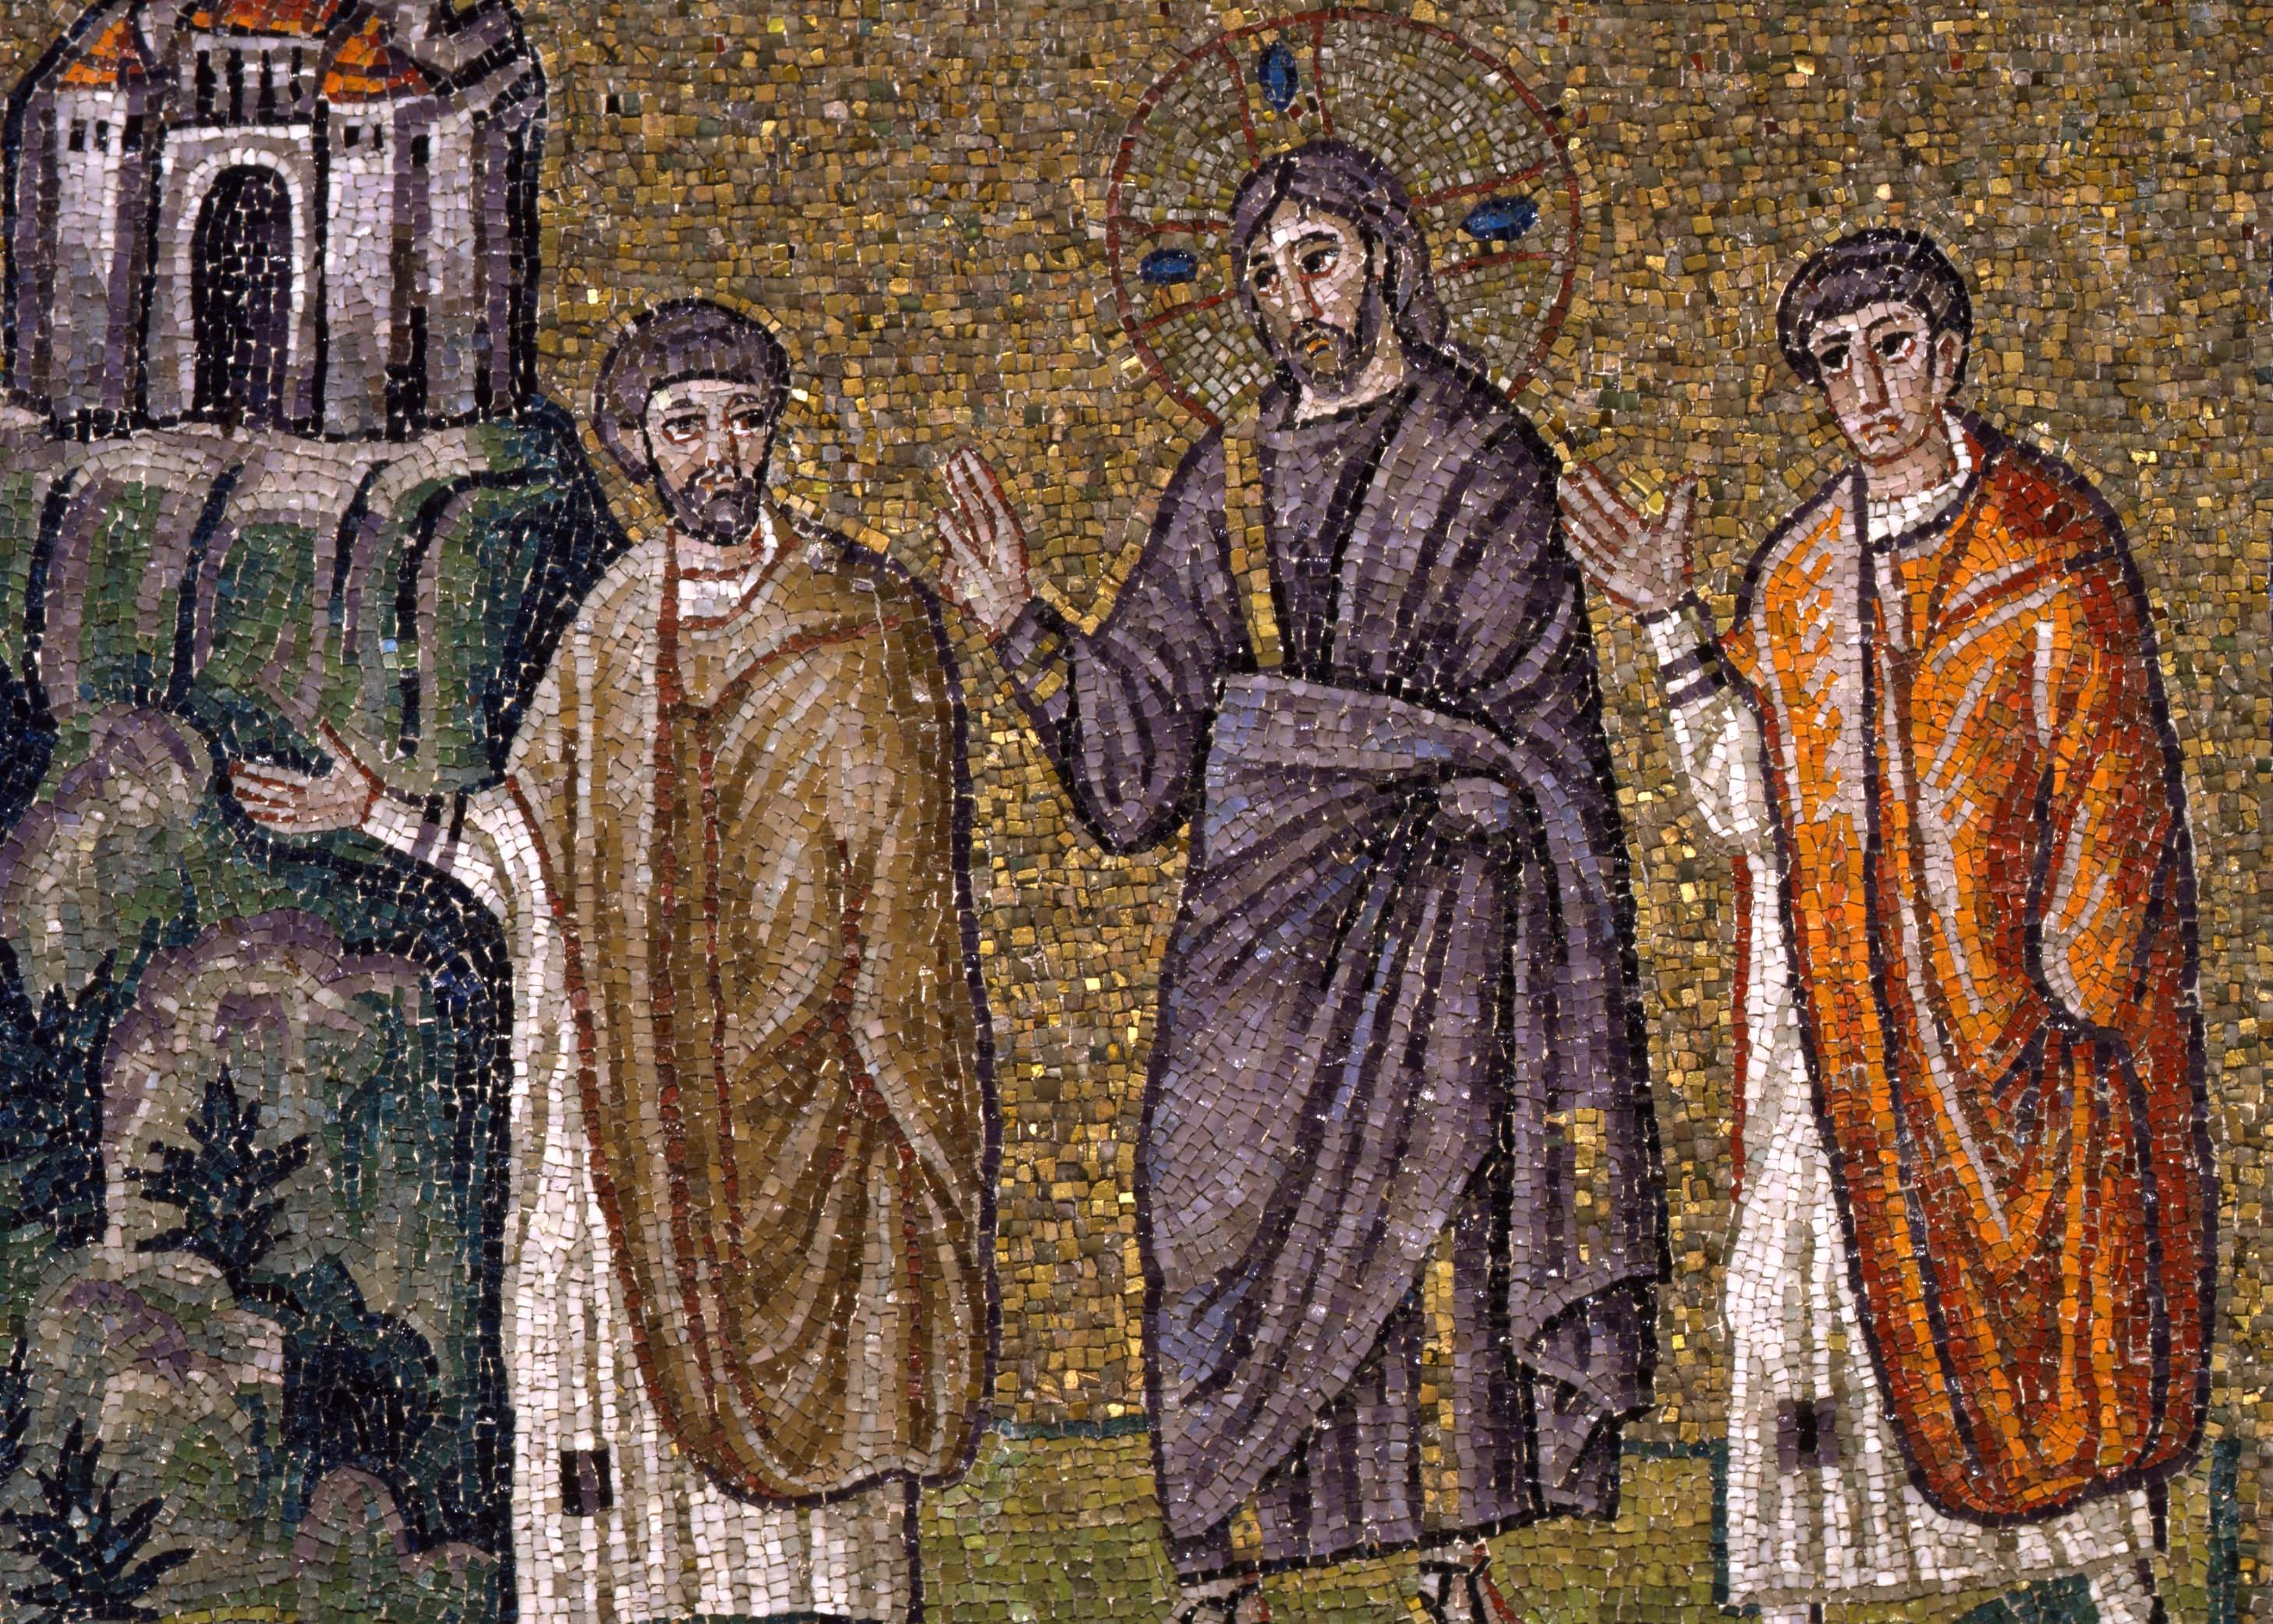
\includegraphics[width=8cm]{emmaus.jpg}
%\end{center}

\vfill

\begin{center}
%Ad usum et secundum consuetudines chori \guillemotright{}Conventus Choralis\guillemotleft.

%Editio Sancti Wolfgangi \annusEditionis
\end{center}

\pagebreak

\renewcommand{\headrulewidth}{0pt} % no horiz. rule at the header
\fancyhf{}
\pagestyle{fancy}

\pars{Oratio ante divinum Officium.}

\lettrine{{\color{red}A}}{peri,} Dómine, os meum ad benedicéndum nomen sanctum tuum:
munda quoque cor meum ab ómnibus vanis, pervérsis, et aliénis
cogitatiónibus:
intelléctum illúmina, afféctum inflámma,
ut digne, atténte ac devóte hoc Offícium recitáre váleam,
et exaudíri mérear ante conspéctum Divínæ Maiestátis tuæ.
Per Christum, Dóminum nostrum.
\Rbardot{} Amen.

Dómine, in unióne illíus divínæ intentiónis,
qua ipse in terris laudes Deo persolvísti,
has tibi Horas \rubricatum{(vel \textnormal{hanc tibi Horam})} persólvo.

%\trOratioAnteOfficium

\vfill

\pars{Oratio post divinum Officium.}

\rubrica{
  Orationem sequentem devote post Officium recitantibus
  Leo Papa X. defectus, et culpas in eo persolvendo ex humana
  fragilitate contractas, indulsit, et dicitur flexis genibus.
}

\lettrine{{\color{red}S}}{acrosánctæ} et indivíduæ Trinitáti,
crucifíxi Dómini nostri Iesu Christi humanitáti,
beatíssimæ et gloriosíssimæ sempérque Vírginis Maríæ
fecúndæ integritáti, 
et ómnium Sanctórum universitáti
sit sempitérna laus, honor, virtus et glória
ab omni creatúra,
nobísque remíssio ómnium peccatórum,
per infiníta sǽcula sæculórum.
\Rbardot{} Amen.

\noindent \Vbardot{} Beáta víscera Maríæ Virginis, quæ portavérunt
ætérni Patris Fílium.\\
\Rbardot{} Et beáta úbera, quæ lactavérunt Christum Dominum.

\rubrica{Et dicitur secreto \textnormal{Pater noster.} et \textnormal{Ave María.}}

%\trOratioPostOfficium

\vfill

\hora{Ad I. Vesperas.} %%%%%%%%%%%%%%%%%%%%%%%%%%%%%%%%%%%%%%%%%%%%%%%%%%%%%
%\sideThumbs{I. Vesperæ}

\cantusSineNeumas

\vspace{0.5cm}
\grechangedim{interwordspacetext}{0.18 cm plus 0.15 cm minus 0.05 cm}{scalable}%
\cuminitiali{}{temporalia/deusinadiutorium-solemnis.gtex}
\grechangedim{interwordspacetext}{0.22 cm plus 0.15 cm minus 0.05 cm}{scalable}%

\vfill
\pagebreak

\pars{Psalmus 1.} \scriptura{Ps. 144, 13; \textbf{H100}}

\vspace{-4mm}

\antiphona{VII c\textsuperscript{2}}{temporalia/ant-regnumtuum.gtex}

\scriptura{Psalmus 144, 10-21.}

\initiumpsalmi{temporalia/ps144ii-initium-vii-c2-auto.gtex}

%\psalmusEtTranslatioT{temporalia/ps144ii-VII-comb.tex}{10cm}
\input{temporalia/ps144ii-VII.tex} \Abardot{}

\vspace{-1cm}

\vfill
\pagebreak

\pars{Psalmus 2.} \scriptura{Ps. 145, 2; \textbf{H100}}

\vspace{-4mm}

\antiphona{IV E}{temporalia/ant-laudabodeum.gtex}

\scriptura{Psalmus 145.}

\initiumpsalmi{temporalia/ps145-initium-iv-E-auto.gtex}

%\psalmusEtTranslatioT{temporalia/ps145-VII-comb.tex}{10cm}
\input{temporalia/ps145-VII.tex} \Abardot{}

\vfill
\pagebreak

\pars{Psalmus 3.} \scriptura{Ps. 146, 1; \textbf{H101}}

\vspace{-4mm}

\antiphona{VIII a}{temporalia/ant-deonostro.gtex}

\scriptura{Psalmus 146.}

\initiumpsalmi{temporalia/ps146-initium-viii-A-auto.gtex}

%\psalmusEtTranslatioT{temporalia/ps146-VII-comb.tex}{10cm}
\input{temporalia/ps146-VII.tex} \Abardot{}

\vfill
\pagebreak

\pars{Psalmus 4.} \scriptura{Ps. 147, 1}

\vspace{-4mm}

\antiphona{E}{temporalia/ant-laudajerusalem.gtex}

\scriptura{Psalmus 147.}

\initiumpsalmi{temporalia/ps147-initium-e-auto.gtex}

%\psalmusEtTranslatioT{temporalia/ps147-VII-comb.tex}{10cm}
\input{temporalia/ps147-VII.tex} \Abardot{}

\vfill
\pagebreak

\pars{Capitulum.} \scriptura{Rom. 11, 33}

\grechangedim{interwordspacetext}{0.12 cm plus 0.15 cm minus 0.05 cm}{scalable}%
\cuminitiali{}{temporalia/capitulum-OAltitudo.gtex}
\grechangedim{interwordspacetext}{0.22 cm plus 0.15 cm minus 0.05 cm}{scalable}

% preklad Jeruz. bible
%\trCapituliI

\vfill

\pars{Responsorium breve.} \scriptura{Ps. 146, 5}

\cuminitiali{VI}{temporalia/resp-magnusdominusnoster.gtex}

%\trResp

\vfill
\pagebreak

\pars{Hymnus} \scriptura{Ambrosius (\olddag{} 397)}

\cuminitiali{I}{temporalia/hym-OLuxBeata-aestivalis.gtex}
\vspace{-3mm}
%\input{hym-OLuxBeata-bohtext.tex}

\vfill
%\pagebreak

\pars{Versus.}

% Versus. %%%
\sineinitiali{temporalia/versus-vespertina.gtex}

%\noindent \trVersus

\vfill
\pagebreak

\magnificati

\vfill
\pagebreak

%\sideThumbs{{\scriptsize{}Fine horarum}}

\anteOrationem

\pagebreak

% Oratio. %%%
\oratioLaudes

\vspace{-1mm}
%\trOrationisI

\vfill

\rubrica{Hebdomadarius dicit iterum Dominus vobiscum, vel cantor dicit:}

\vspace{2mm}

\sineinitiali{temporalia/domineexaudi.gtex}

\rubrica{Postea cantatur a cantore:}

\vspace{2mm}

\cuminitiali{I}{temporalia/benedicamus-dominica-perannum.gtex}

\vspace{1mm}

\vfill
\pagebreak

\hora{Ad Matutinum.} %%%%%%%%%%%%%%%%%%%%%%%%%%%%%%%%%%%%%%%%%%%%%%%%%%%%%
%\sideThumbs{Matutinum}

\vspace{2mm}

\cuminitiali{}{temporalia/dominelabiamea.gtex}

\vspace{2mm}

\pars{Invitatorium.} \scriptura{Ps. 94, 1; Psalmus 94}

\vspace{-6mm}

\antiphona{E}{temporalia/inv-veniteexsultemus.gtex}

\vfill
\pagebreak

\pars{Hymnus.} \scriptura{Adamus Sancti Victoris (\olddag 1146)}

\vspace{-5mm}

\antiphona{VII}{temporalia/hym-SalveDies.gtex}

\scriptura{Non dicitur \textnormal{Amen} in fine.}
%{
%\vspace{-5mm}
%\setlength{\columnsep}{0pt} % prostor mezi sloupci
%\input{hym-SalveDies-bohtext.tex}
%\setlength{\columnsep}{30pt} % prostor mezi sloupci
%}

\vfill
\pagebreak

\iffalse
\subhora{In I. Nocturno}

\pars{Psalmus 1.} \scriptura{\textbf{H230}}

%\vspace{-5mm}

\antiphona{V a}{temporalia/ant-alleluialapis.gtex}

%\vspace{-5mm}

\scriptura{Ps. 1}

%\vspace{-2mm}

\initiumpsalmi{temporalia/ps1-initium-v-a-auto.gtex}

%\psalmusEtTranslatioT{temporalia/ps1-comb.tex}{10cm}

\input{temporalia/ps1.tex}

\vfill
\pagebreak

\pars{Psalmus 2.}

\scriptura{Ps. 2}

\initiumpsalmi{temporalia/ps2-initium-v-a-auto.gtex}

%\psalmusEtTranslatioT{temporalia/ps2-comb.tex}{10cm}

\input{temporalia/ps2.tex}

\vfill
\pagebreak

\pars{Psalmus 3.}

\scriptura{Ps. 3}

\initiumpsalmi{temporalia/ps3-initium-v-a-auto.gtex}

%\psalmusEtTranslatioT{temporalia/ps3-comb.tex}{10cm}

\input{temporalia/ps3.tex}

\vfill

\antiphona{}{temporalia/ant-alleluialapis.gtex}

\vfill
\pagebreak
\fi

\noindent \Vbardot{} Memor fui nocte nóminis tui, Dómine.
\noindent \Rbardot{} Et custodívi legem tuam.

\vspace{5mm}

\sineinitiali{temporalia/oratiodominica-mat.gtex}

\vspace{5mm}

\pars{Absolutio.}

\cuminitiali{}{temporalia/absolutio-exaudi.gtex}

\vfill
\pagebreak

\cuminitiali{}{temporalia/benedictio-solemn-benedictione.gtex}

\vspace{7mm}

\lectioi

\noindent \Vbardot{} Tu autem, Dómine, miserére nobis.
\noindent \Rbardot{} Deo grátias.

\vfill
\pagebreak

\responsoriumi

\vfill
\pagebreak

\cuminitiali{}{temporalia/benedictio-solemn-unigenitus.gtex}

\vspace{7mm}

\lectioii

\noindent \Vbardot{} Tu autem, Dómine, miserére nobis.
\noindent \Rbardot{} Deo grátias.

\vfill
\pagebreak

\responsoriumii

\vfill
\pagebreak

\cuminitiali{}{temporalia/benedictio-solemn-spiritus.gtex}

\vspace{7mm}

\lectioiii

\noindent \Vbardot{} Tu autem, Dómine, miserére nobis.
\noindent \Rbardot{} Deo grátias.

\vfill
\pagebreak

\responsoriumiii

\vfill
\pagebreak

\iffalse
\subhora{In II. Nocturno}

\pars{Psalmus 4.} \scriptura{Io. 20, 15; \textbf{H241}}

%\vspace{-5mm}

\antiphona{V a}{temporalia/ant-alleluiaquem.gtex}

%\vspace{-5mm}

\scriptura{Ps. 8}

%A\vspace{-2mm}

\initiumpsalmi{temporalia/ps8-initium-v-a-auto.gtex}

%\psalmusEtTranslatioT{temporalia/ps8-comb.tex}{10cm}

\input{temporalia/ps8.tex}

\vfill
\pagebreak

\pars{Psalmus 5.}

\scriptura{Ps. 9, 2-11}

\initiumpsalmi{temporalia/ps9ii_xi-initium-v-a-auto.gtex}

%\psalmusEtTranslatioT{temporalia/ps9ii_xi-comb.tex}{10cm}

\input{temporalia/ps9ii_xi.tex}

\vfill
\pagebreak

\pars{Psalmus 6.}

\scriptura{Ps. 9, 12-21}

\initiumpsalmi{temporalia/ps9xii_xxi-initium-v-a-auto.gtex}

%\psalmusEtTranslatioT{temporalia/ps9xii_xxi-comb.tex}{10cm}

\input{temporalia/ps9xii_xxi.tex}

\vfill

\antiphona{}{temporalia/ant-alleluiaquem.gtex}

\vfill
\pagebreak
\fi

\noindent \Vbardot{} Média nocte surgébam ad confiténdum tibi.
\noindent \Rbardot{} Super iudícia iustificatiónis tuæ.

\vspace{5mm}

\sineinitiali{temporalia/oratiodominica-mat.gtex}

\vspace{5mm}

\pars{Absolutio.}

\cuminitiali{}{temporalia/absolutio-ipsius.gtex}

\vfill
\pagebreak

\cuminitiali{}{temporalia/benedictio-solemn-deus.gtex}

\vspace{7mm}

\lectioiv

\noindent \Vbardot{} Tu autem, Dómine, miserére nobis.
\noindent \Rbardot{} Deo grátias.

\vfill
\pagebreak

\responsoriumiv

\vfill
\pagebreak

\cuminitiali{}{temporalia/benedictio-solemn-christus.gtex}

\vspace{7mm}

\lectiov

\noindent \Vbardot{} Tu autem, Dómine, miserére nobis.
\noindent \Rbardot{} Deo grátias.

\vfill
\pagebreak

\responsoriumv

\vfill
\pagebreak

\cuminitiali{}{temporalia/benedictio-solemn-ignem.gtex}

\vspace{7mm}

\lectiovi

\noindent \Vbardot{} Tu autem, Dómine, miserére nobis.
\noindent \Rbardot{} Deo grátias.

\vfill
\pagebreak

\responsoriumvi

\vfill
\pagebreak

\iffalse
\subhora{In III. Nocturno}

\pars{Psalmus 7.} \scriptura{Cf. Io. 20, 15; \textbf{H241}}

\vspace{-5mm}

\antiphona{V a}{temporalia/ant-alleluianoli.gtex}

\vspace{-4mm}

\scriptura{Ps. 9, 22-32}

%\vspace{-2mm}

\initiumpsalmi{temporalia/ps9xxii_xxxii-initium-v-a-auto.gtex}

%\psalmusEtTranslatioT{temporalia/ps9xxii_xxxii-comb.tex}{10cm}

\input{temporalia/ps9xxii_xxxii.tex}

\vfill
\pagebreak

\pars{Psalmus 8.}

\scriptura{Ps. 9, 33-39}

\initiumpsalmi{temporalia/ps9xxxiii_xxxix-initium-v-a-auto.gtex}

%\psalmusEtTranslatioT{temporalia/ps9xxxiii_xxxix-comb.tex}{10cm}

\input{temporalia/ps9xxxiii_xxxix.tex}

\vfill
\pagebreak

\pars{Psalmus 9.}

\scriptura{Ps. 10}

\initiumpsalmi{temporalia/ps10-initium-v-a-auto.gtex}

%\psalmusEtTranslatioT{temporalia/ps10-comb.tex}{10cm}

\input{temporalia/ps10.tex}

\vfill

\antiphona{}{temporalia/ant-alleluianoli.gtex}

\vfill
\pagebreak
\fi

\noindent \Vbardot{} Prævenérunt óculi mei ad te dilúculo.
\noindent \Rbardot{} Ut meditárer elóquia tua, Dómine.

\vspace{5mm}

\sineinitiali{temporalia/oratiodominica-mat.gtex}

\vspace{5mm}

\pars{Absolutio.}

\cuminitiali{}{temporalia/absolutio-avinculis.gtex}

\vfill
\pagebreak

\cuminitiali{}{temporalia/benedictio-solemn-evangelica.gtex}

\vspace{7mm}

\lectiovii

\noindent \Vbardot{} Tu autem, Dómine, miserére nobis.
\noindent \Rbardot{} Deo grátias.

\vfill
\pagebreak

\responsoriumvii

\vfill
\pagebreak

\cuminitiali{}{temporalia/benedictio-solemn-divinum.gtex}

\vspace{7mm}

\lectioviii

\noindent \Vbardot{} Tu autem, Dómine, miserére nobis.
\noindent \Rbardot{} Deo grátias.

\vfill
\pagebreak

\responsoriumviii

\vfill
\pagebreak

\cuminitiali{}{temporalia/benedictio-solemn-adsocietatem.gtex}

\vspace{7mm}

\lectioix

\noindent \Vbardot{} Tu autem, Dómine, miserére nobis.
\noindent \Rbardot{} Deo grátias.

\vfill
\pagebreak

% Te Deum

{
\pars{Hymnus Ambrosianus} \scriptura{Tonus Solemnis}

\vspace{-2mm}

\grechangedim{interwordspacetext}{0.26 cm plus 0.15 cm minus 0.05 cm}{scalable}%
\cuminitiali{III}{temporalia/tedeum-solemnis-gn.gtex}
\grechangedim{interwordspacetext}{0.22 cm plus 0.15 cm minus 0.05 cm}{scalable}%
}

\vfill
\pagebreak

\rubrica{Reliqua omittuntur, nisi Laudes separandæ sint.}

\pars{Oratio}

\noindent \Vbardot{} Dómine, exáudi oratiónem meam.

\noindent \Rbardot{} Et clamor meus ad te véniat.

Orémus:

\oratioLaudes

\vspace{7mm}

\pars{Conclusio}

\noindent \Vbardot{} Dómine, exáudi oratiónem meam.

\noindent \Rbardot{} Et clamor meus ad te véniat.

\noindent \Vbardot{} Benedicámus Dómino, allelúia, allelúia.

\noindent \Rbardot{} Deo grátias, allelúia, allelúia.

\noindent \Vbardot{} Fidélium ánimæ per misericórdiam Dei requiéscant in pace.

\noindent \Rbardot{} Amen.

\vfill
\pagebreak

\hora{Ad Laudes.} %%%%%%%%%%%%%%%%%%%%%%%%%%%%%%%%%%%%%%%%%%%%%%%%%%%%%
%\sideThumbs{Laudes}

\cantusSineNeumas

\vspace{0.5cm}
\grechangedim{interwordspacetext}{0.18 cm plus 0.15 cm minus 0.05 cm}{scalable}%
\cuminitiali{}{temporalia/deusinadiutorium-alter.gtex}
\grechangedim{interwordspacetext}{0.22 cm plus 0.15 cm minus 0.05 cm}{scalable}%

\vfill
%\pagebreak

\pars{Psalmus 1.}

\vspace{-4mm}

\antiphona{VI F}{temporalia/ant-alleluia1.gtex}

\scriptura{Psalmus 50.}

\initiumpsalmi{temporalia/ps50-initium-vi-F-auto.gtex}

%\psalmusEtTranslatioT{temporalia/ps50-I-comb.tex}{10cm}
\input{temporalia/ps50-I.tex}

\vfill
\pagebreak

\pars{Psalmus 2.}

\scriptura{Psalmus 117.}

\initiumpsalmi{temporalia/ps117-initium-vi-F-auto.gtex}

%\psalmusEtTranslatioT{temporalia/ps117-I-comb.tex}{10cm}
\input{temporalia/ps117-I.tex}

\vfill
\pagebreak

\pars{Psalmus 3.}

\scriptura{Psalmus 62.}

\initiumpsalmi{temporalia/ps62-initium-vi-F-auto.gtex}

%\psalmusEtTranslatioT{temporalia/ps62-I-comb.tex}{10cm}
\input{temporalia/ps62-I.tex}

\vfill

\vspace{-6mm}

\antiphona{}{temporalia/ant-alleluia1.gtex} % repeat the antiphon - new page

\vfill
\pagebreak

\pars{Psalmus 4.} \scriptura{Dan. 3, 22-26; \textbf{H422}}

\vspace{-4mm}

\antiphona{VIII G}{temporalia/ant-trespueri.gtex}

\scriptura{Canticum trium puerorum, Dan. 3, 57-88 et 56}

\initiumpsalmi{temporalia/dan3-initium-viii-G-auto.gtex}

%\psalmusEtTranslatioT{temporalia/dan3-comb.tex}{10cm}
\input{temporalia/dan3.tex}

\rubrica{Hic non dicitur Gloria Patri, neque Amen.}

\vfill

\vspace{-6mm}

\antiphona{}{temporalia/ant-trespueri.gtex} % repeat the antiphon - new page

\vfill
\pagebreak

\pars{Psalmus 5.}

\vspace{-4mm}

\antiphona{VIII G}{temporalia/ant-alleluia2.gtex}

\scriptura{Psalmus 148.}

\initiumpsalmi{temporalia/ps148-initium-viii-G-auto.gtex}

%\psalmusEtTranslatioT{temporalia/ps148-I-comb.tex}{10cm}
\input{temporalia/ps148-I.tex}

\rubrica{Hic non dicitur Gloria Patri.}

\vfill
\pagebreak

%
\scriptura{Psalmus 149.}

\initiumpsalmi{temporalia/ps149-initium-viii-G-auto.gtex}

%\psalmusEtTranslatioT{temporalia/ps149-I-comb.tex}{10cm}
\input{temporalia/ps149-I.tex}

\rubrica{Hic non dicitur Gloria Patri.}

\vfill
\pagebreak

%
\scriptura{Psalmus 150.}

\initiumpsalmi{temporalia/ps150-initium-viii-G-auto.gtex}

%\psalmusEtTranslatioT{temporalia/ps150-I-comb.tex}{10cm}
\input{temporalia/ps150-I.tex}

\vfill

\vspace{-6mm}

\antiphona{}{temporalia/ant-alleluia2.gtex} % repeat the antiphon - new page

\vfill
\pagebreak

\pars{Capitulum.} \scriptura{Ac. 7, 12}

\grechangedim{interwordspacetext}{0.12 cm plus 0.15 cm minus 0.05 cm}{scalable}%
\cuminitiali{}{temporalia/capitulum-Benedictio.gtex}
\grechangedim{interwordspacetext}{0.22 cm plus 0.15 cm minus 0.05 cm}{scalable}

% preklad Jeruz. bible
%\trCapituliI

\vfill

\pars{Responsorium breve.} \scriptura{Ps. 118, 36-37}

\cuminitiali{IV}{temporalia/resp-inclinacormeum.gtex}

%\trResp

\vfill
\pagebreak

\pars{Hymnus} \scriptura{Gregorius Magnus (\olddag{} 604)}

\cuminitiali{IV}{temporalia/hym-EcceJamNoctis.gtex}
\vspace{-3mm}
%\input{hym-EcceJamNocis-bohtext.tex}

\vfill
%\pagebreak

\pars{Versus.} \scriptura{Ps. 92, 1}

% Versus. %%%
\sineinitiali{temporalia/versus-dominusregnavit.gtex}

%\noindent \trVersus

\vfill
\pagebreak

\benedictus

\vspace{-1cm}

\vfill
\pagebreak

%\sideThumbs{{\scriptsize{}Fine horarum}}

\anteOrationem

\pagebreak

% Oratio. %%%
\oratioLaudes

\vspace{-1mm}
%\trOrationisI

\vfill

\rubrica{Hebdomadarius dicit iterum Dominus vobiscum, vel cantor dicit:}

\vspace{2mm}

\sineinitiali{temporalia/domineexaudi.gtex}

\rubrica{Postea cantatur a cantore:}

\vspace{2mm}

\cuminitiali{I}{temporalia/benedicamus-dominica-perannum.gtex}

\vspace{1mm}

\vfill
\pagebreak

\hora{Ad II. Vesperas.} %%%%%%%%%%%%%%%%%%%%%%%%%%%%%%%%%%%%%%%%%%%%%%%%%%%%%
%\sideThumbs{II. Vesperæ}

\cantusSineNeumas

%\vspace{0.5cm}
\grechangedim{interwordspacetext}{0.18 cm plus 0.15 cm minus 0.05 cm}{scalable}%
\cuminitiali{}{temporalia/deusinadiutorium-solemnis.gtex}
\grechangedim{interwordspacetext}{0.22 cm plus 0.15 cm minus 0.05 cm}{scalable}%

\vfill
%\pagebreak

\vspace{-2mm}

\pars{Psalmus 1.} \scriptura{Ps. 109, 1; \textbf{H91}}

\vspace{-4mm}

\antiphona{VII c\textsuperscript{2}}{temporalia/ant-dixitdominus.gtex}

\vspace{-4mm}

\scriptura{Psalmus 109.}

\initiumpsalmi{temporalia/ps109-initium-vii-c2-auto.gtex}

%\psalmusEtTranslatioT{temporalia/ps109-I-comb.tex}{10cm}
\input{temporalia/ps109-I.tex} \Abardot{}

\vspace{-1cm}

\vfill
\pagebreak

\pars{Psalmus 2.} \scriptura{Ps. 110, 8; \textbf{H91}}

\vspace{-4mm}

\antiphona{IV g}{temporalia/ant-fideliaomnia.gtex}

\scriptura{Psalmus 110.}

\initiumpsalmi{temporalia/ps110-initium-iv-g-auto.gtex}

%\psalmusEtTranslatioT{temporalia/ps110-I-comb.tex}{10cm}
\input{temporalia/ps110-I.tex} \Abardot{}

\vfill
\pagebreak

\pars{Psalmus 3.} \scriptura{Ps. 111, 1; \textbf{H92}}

\vspace{-4mm}

\antiphona{IV a}{temporalia/ant-inmandatis.gtex}

\scriptura{Psalmus 111.}

\initiumpsalmi{temporalia/ps111-initium-iv-a-auto.gtex}

%\psalmusEtTranslatioT{temporalia/ps111-I-comb.tex}{10cm}
\input{temporalia/ps111-I.tex} \Abardot{}

\vfill
\pagebreak

\pars{Psalmus 4.} \scriptura{Ps. 112, 2; \textbf{H92}}

\vspace{-4mm}

\antiphona{VII c}{temporalia/ant-sitnomendomini.gtex}

\scriptura{Psalmus 112.}

\initiumpsalmi{temporalia/ps112-initium-vii-c-auto.gtex}

%\psalmusEtTranslatioT{temporalia/ps112-I-comb.tex}{10cm}
\input{temporalia/ps112-I.tex} \Abardot{}

\vfill
\pagebreak

\pars{Capitulum.} \scriptura{2 Cor. 1, 3-4}

\grechangedim{interwordspacetext}{0.12 cm plus 0.15 cm minus 0.05 cm}{scalable}%
\cuminitiali{}{temporalia/capitulum-BenedictusDeus.gtex}
\grechangedim{interwordspacetext}{0.22 cm plus 0.15 cm minus 0.05 cm}{scalable}

% preklad Jeruz. bible
%\trCapituliI

\vfill

\pars{Responsorium breve.} \scriptura{Ps. 103, 24}

\cuminitiali{VI}{temporalia/resp-quammagnificata.gtex}

%\trResp

\vfill
\pagebreak

\pars{Hymnus} \scriptura{Gregorius Magnus (\olddag{} 604)}

\cuminitiali{I}{temporalia/hym-LucisCreator-aestivalis.gtex}
\vspace{-3mm}
%\begin{translatioMulticol}{3}
Tvůrce světa předobrý,\\
tys ustanovil denní řád\\
a proudy světla rozhodil,\\
když světu základy jsi klad.\\
\\
A spojils ráno s večerem\\
a dnem tu dobu nazýváš;\\
hle padá temné noci stín -\\
slyš prosbu, vyslyš nářek náš.\columnbreak

Ach, nedej, by nás stihla smrt,\\
když svědomí nám tíží hřích,\\
když nemyslíme na věčnost\\
v té síti hříchů šalebných.\\
\\
Vzbuď naši touhu po nebi,\\
kde věčný život čeká nás,\\
a pomoz odložit vše zlé\\
a smýti z duše každý kaz.\columnbreak

To splň nám, dobrý Otče náš,\\
i ty, jenž rovné božství máš,\\
i Duchu, který těšíš nás\\
a vládneš, Bože, v každý čas.\\
Amen. 
\end{translatioMulticol}


\vfill
%\pagebreak

\pars{Versus.} \scriptura{Ps. 140, 2}

% Versus. %%%
\sineinitiali{temporalia/versus-dirigatur.gtex}

%\noindent \trVersus

\vfill
\pagebreak

\magnificatii

\vfill
\pagebreak

%\sideThumbs{{\scriptsize{}Fine horarum}}

\anteOrationem

\pagebreak

% Oratio. %%%
\oratioLaudes

\vspace{-1mm}
%\trOrationisI

\vfill

\rubrica{Hebdomadarius dicit iterum Dominus vobiscum, vel cantor dicit:}

\vspace{2mm}

\sineinitiali{temporalia/domineexaudi.gtex}

\rubrica{Postea cantatur a cantore:}

\vspace{2mm}

\cuminitiali{I}{temporalia/benedicamus-dominica-perannum.gtex}

\vspace{1mm}

\end{document}

